% Options for packages loaded elsewhere
\PassOptionsToPackage{unicode}{hyperref}
\PassOptionsToPackage{hyphens}{url}
%
\documentclass[
]{article}
\usepackage{lmodern}
\usepackage{amssymb,amsmath}
\usepackage{ifxetex,ifluatex}
\ifnum 0\ifxetex 1\fi\ifluatex 1\fi=0 % if pdftex
  \usepackage[T1]{fontenc}
  \usepackage[utf8]{inputenc}
  \usepackage{textcomp} % provide euro and other symbols
\else % if luatex or xetex
  \usepackage{unicode-math}
  \defaultfontfeatures{Scale=MatchLowercase}
  \defaultfontfeatures[\rmfamily]{Ligatures=TeX,Scale=1}
\fi
% Use upquote if available, for straight quotes in verbatim environments
\IfFileExists{upquote.sty}{\usepackage{upquote}}{}
\IfFileExists{microtype.sty}{% use microtype if available
  \usepackage[]{microtype}
  \UseMicrotypeSet[protrusion]{basicmath} % disable protrusion for tt fonts
}{}
\makeatletter
\@ifundefined{KOMAClassName}{% if non-KOMA class
  \IfFileExists{parskip.sty}{%
    \usepackage{parskip}
  }{% else
    \setlength{\parindent}{0pt}
    \setlength{\parskip}{6pt plus 2pt minus 1pt}}
}{% if KOMA class
  \KOMAoptions{parskip=half}}
\makeatother
\usepackage{xcolor}
\IfFileExists{xurl.sty}{\usepackage{xurl}}{} % add URL line breaks if available
\IfFileExists{bookmark.sty}{\usepackage{bookmark}}{\usepackage{hyperref}}
\hypersetup{
  pdftitle={IBM HR Analytics ML Classification},
  pdfauthor={Yevonnael Andrew},
  hidelinks,
  pdfcreator={LaTeX via pandoc}}
\urlstyle{same} % disable monospaced font for URLs
\usepackage[margin=1in]{geometry}
\usepackage{color}
\usepackage{fancyvrb}
\newcommand{\VerbBar}{|}
\newcommand{\VERB}{\Verb[commandchars=\\\{\}]}
\DefineVerbatimEnvironment{Highlighting}{Verbatim}{commandchars=\\\{\}}
% Add ',fontsize=\small' for more characters per line
\usepackage{framed}
\definecolor{shadecolor}{RGB}{248,248,248}
\newenvironment{Shaded}{\begin{snugshade}}{\end{snugshade}}
\newcommand{\AlertTok}[1]{\textcolor[rgb]{0.94,0.16,0.16}{#1}}
\newcommand{\AnnotationTok}[1]{\textcolor[rgb]{0.56,0.35,0.01}{\textbf{\textit{#1}}}}
\newcommand{\AttributeTok}[1]{\textcolor[rgb]{0.77,0.63,0.00}{#1}}
\newcommand{\BaseNTok}[1]{\textcolor[rgb]{0.00,0.00,0.81}{#1}}
\newcommand{\BuiltInTok}[1]{#1}
\newcommand{\CharTok}[1]{\textcolor[rgb]{0.31,0.60,0.02}{#1}}
\newcommand{\CommentTok}[1]{\textcolor[rgb]{0.56,0.35,0.01}{\textit{#1}}}
\newcommand{\CommentVarTok}[1]{\textcolor[rgb]{0.56,0.35,0.01}{\textbf{\textit{#1}}}}
\newcommand{\ConstantTok}[1]{\textcolor[rgb]{0.00,0.00,0.00}{#1}}
\newcommand{\ControlFlowTok}[1]{\textcolor[rgb]{0.13,0.29,0.53}{\textbf{#1}}}
\newcommand{\DataTypeTok}[1]{\textcolor[rgb]{0.13,0.29,0.53}{#1}}
\newcommand{\DecValTok}[1]{\textcolor[rgb]{0.00,0.00,0.81}{#1}}
\newcommand{\DocumentationTok}[1]{\textcolor[rgb]{0.56,0.35,0.01}{\textbf{\textit{#1}}}}
\newcommand{\ErrorTok}[1]{\textcolor[rgb]{0.64,0.00,0.00}{\textbf{#1}}}
\newcommand{\ExtensionTok}[1]{#1}
\newcommand{\FloatTok}[1]{\textcolor[rgb]{0.00,0.00,0.81}{#1}}
\newcommand{\FunctionTok}[1]{\textcolor[rgb]{0.00,0.00,0.00}{#1}}
\newcommand{\ImportTok}[1]{#1}
\newcommand{\InformationTok}[1]{\textcolor[rgb]{0.56,0.35,0.01}{\textbf{\textit{#1}}}}
\newcommand{\KeywordTok}[1]{\textcolor[rgb]{0.13,0.29,0.53}{\textbf{#1}}}
\newcommand{\NormalTok}[1]{#1}
\newcommand{\OperatorTok}[1]{\textcolor[rgb]{0.81,0.36,0.00}{\textbf{#1}}}
\newcommand{\OtherTok}[1]{\textcolor[rgb]{0.56,0.35,0.01}{#1}}
\newcommand{\PreprocessorTok}[1]{\textcolor[rgb]{0.56,0.35,0.01}{\textit{#1}}}
\newcommand{\RegionMarkerTok}[1]{#1}
\newcommand{\SpecialCharTok}[1]{\textcolor[rgb]{0.00,0.00,0.00}{#1}}
\newcommand{\SpecialStringTok}[1]{\textcolor[rgb]{0.31,0.60,0.02}{#1}}
\newcommand{\StringTok}[1]{\textcolor[rgb]{0.31,0.60,0.02}{#1}}
\newcommand{\VariableTok}[1]{\textcolor[rgb]{0.00,0.00,0.00}{#1}}
\newcommand{\VerbatimStringTok}[1]{\textcolor[rgb]{0.31,0.60,0.02}{#1}}
\newcommand{\WarningTok}[1]{\textcolor[rgb]{0.56,0.35,0.01}{\textbf{\textit{#1}}}}
\usepackage{longtable,booktabs}
% Correct order of tables after \paragraph or \subparagraph
\usepackage{etoolbox}
\makeatletter
\patchcmd\longtable{\par}{\if@noskipsec\mbox{}\fi\par}{}{}
\makeatother
% Allow footnotes in longtable head/foot
\IfFileExists{footnotehyper.sty}{\usepackage{footnotehyper}}{\usepackage{footnote}}
\makesavenoteenv{longtable}
\usepackage{graphicx,grffile}
\makeatletter
\def\maxwidth{\ifdim\Gin@nat@width>\linewidth\linewidth\else\Gin@nat@width\fi}
\def\maxheight{\ifdim\Gin@nat@height>\textheight\textheight\else\Gin@nat@height\fi}
\makeatother
% Scale images if necessary, so that they will not overflow the page
% margins by default, and it is still possible to overwrite the defaults
% using explicit options in \includegraphics[width, height, ...]{}
\setkeys{Gin}{width=\maxwidth,height=\maxheight,keepaspectratio}
% Set default figure placement to htbp
\makeatletter
\def\fps@figure{htbp}
\makeatother
\setlength{\emergencystretch}{3em} % prevent overfull lines
\providecommand{\tightlist}{%
  \setlength{\itemsep}{0pt}\setlength{\parskip}{0pt}}
\setcounter{secnumdepth}{-\maxdimen} % remove section numbering

\title{IBM HR Analytics ML Classification}
\author{Yevonnael Andrew}
\date{2/5/2020}

\begin{document}
\maketitle

\hypertarget{introduction}{%
\section{Introduction}\label{introduction}}

This analysis will try to classify the Attrition of the given employee.
The dataset is downloaded from Kaggle:
\url{https://www.kaggle.com/pavansubhasht/ibm-hr-analytics-attrition-dataset}

This analysis is part of Algoritma LBB Project in C1 class. In this
project, I will create a logistic regression model and a KNN model with
different parameter and tuning, and compare them which predict better
for this dataset.

\begin{Shaded}
\begin{Highlighting}[]
\KeywordTok{library}\NormalTok{(tidyverse)}
\KeywordTok{library}\NormalTok{(plotly)}
\KeywordTok{library}\NormalTok{(ggpubr)}
\KeywordTok{library}\NormalTok{(scales)}
\KeywordTok{library}\NormalTok{(skimr)}
\KeywordTok{library}\NormalTok{(GGally)}
\KeywordTok{library}\NormalTok{(corrr)}
\KeywordTok{library}\NormalTok{(corrplot)}
\KeywordTok{library}\NormalTok{(brglm2)}
\KeywordTok{library}\NormalTok{(ROSE)}
\KeywordTok{library}\NormalTok{(ROCR)}
\KeywordTok{library}\NormalTok{(caret)}
\end{Highlighting}
\end{Shaded}

\begin{Shaded}
\begin{Highlighting}[]
\NormalTok{dataHR <-}\StringTok{ }\KeywordTok{read.csv}\NormalTok{(}\DataTypeTok{file =} \StringTok{'WA_Fn-UseC_-HR-Employee-Attrition.csv'}\NormalTok{)}
\end{Highlighting}
\end{Shaded}

Now we will get a glimpse over the data. Personally I like the skim()
function from skimr package over glimpse() or summary() because it give
a more detailed information about the data, including the missing rate,
complete rate, number of unique, column type and for the numeric type,
it return the five-number summary with a cute little histogram.

\begin{Shaded}
\begin{Highlighting}[]
\KeywordTok{skim}\NormalTok{(dataHR)}
\end{Highlighting}
\end{Shaded}

\begin{longtable}[]{@{}ll@{}}
\caption{Data summary}\tabularnewline
\toprule
\endhead
Name & dataHR\tabularnewline
Number of rows & 1470\tabularnewline
Number of columns & 35\tabularnewline
\_\_\_\_\_\_\_\_\_\_\_\_\_\_\_\_\_\_\_\_\_\_\_ &\tabularnewline
Column type frequency: &\tabularnewline
factor & 9\tabularnewline
numeric & 26\tabularnewline
\_\_\_\_\_\_\_\_\_\_\_\_\_\_\_\_\_\_\_\_\_\_\_\_ &\tabularnewline
Group variables & None\tabularnewline
\bottomrule
\end{longtable}

\textbf{Variable type: factor}

\begin{longtable}[]{@{}lrrlrl@{}}
\toprule
skim\_variable & n\_missing & complete\_rate & ordered & n\_unique &
top\_counts\tabularnewline
\midrule
\endhead
Attrition & 0 & 1 & FALSE & 2 & No: 1233, Yes: 237\tabularnewline
BusinessTravel & 0 & 1 & FALSE & 3 & Tra: 1043, Tra: 277, Non:
150\tabularnewline
Department & 0 & 1 & FALSE & 3 & Res: 961, Sal: 446, Hum:
63\tabularnewline
EducationField & 0 & 1 & FALSE & 6 & Lif: 606, Med: 464, Mar: 159, Tec:
132\tabularnewline
Gender & 0 & 1 & FALSE & 2 & Mal: 882, Fem: 588\tabularnewline
JobRole & 0 & 1 & FALSE & 9 & Sal: 326, Res: 292, Lab: 259, Man:
145\tabularnewline
MaritalStatus & 0 & 1 & FALSE & 3 & Mar: 673, Sin: 470, Div:
327\tabularnewline
Over18 & 0 & 1 & FALSE & 1 & Y: 1470\tabularnewline
OverTime & 0 & 1 & FALSE & 2 & No: 1054, Yes: 416\tabularnewline
\bottomrule
\end{longtable}

\textbf{Variable type: numeric}

\begin{longtable}[]{@{}lrrrrrrrrrl@{}}
\toprule
skim\_variable & n\_missing & complete\_rate & mean & sd & p0 & p25 &
p50 & p75 & p100 & hist\tabularnewline
\midrule
\endhead
ï..Age & 0 & 1 & 36.92 & 9.14 & 18 & 30.00 & 36.0 & 43.00 & 60 &
▂▇▇▃▂\tabularnewline
DailyRate & 0 & 1 & 802.49 & 403.51 & 102 & 465.00 & 802.0 & 1157.00 &
1499 & ▇▇▇▇▇\tabularnewline
DistanceFromHome & 0 & 1 & 9.19 & 8.11 & 1 & 2.00 & 7.0 & 14.00 & 29 &
▇▅▂▂▂\tabularnewline
Education & 0 & 1 & 2.91 & 1.02 & 1 & 2.00 & 3.0 & 4.00 & 5 &
▂▃▇▆▁\tabularnewline
EmployeeCount & 0 & 1 & 1.00 & 0.00 & 1 & 1.00 & 1.0 & 1.00 & 1 &
▁▁▇▁▁\tabularnewline
EmployeeNumber & 0 & 1 & 1024.87 & 602.02 & 1 & 491.25 & 1020.5 &
1555.75 & 2068 & ▇▇▇▇▇\tabularnewline
EnvironmentSatisfaction & 0 & 1 & 2.72 & 1.09 & 1 & 2.00 & 3.0 & 4.00 &
4 & ▅▅▁▇▇\tabularnewline
HourlyRate & 0 & 1 & 65.89 & 20.33 & 30 & 48.00 & 66.0 & 83.75 & 100 &
▇▇▇▇▇\tabularnewline
JobInvolvement & 0 & 1 & 2.73 & 0.71 & 1 & 2.00 & 3.0 & 3.00 & 4 &
▁▃▁▇▁\tabularnewline
JobLevel & 0 & 1 & 2.06 & 1.11 & 1 & 1.00 & 2.0 & 3.00 & 5 &
▇▇▃▂▁\tabularnewline
JobSatisfaction & 0 & 1 & 2.73 & 1.10 & 1 & 2.00 & 3.0 & 4.00 & 4 &
▅▅▁▇▇\tabularnewline
MonthlyIncome & 0 & 1 & 6502.93 & 4707.96 & 1009 & 2911.00 & 4919.0 &
8379.00 & 19999 & ▇▅▂▁▂\tabularnewline
MonthlyRate & 0 & 1 & 14313.10 & 7117.79 & 2094 & 8047.00 & 14235.5 &
20461.50 & 26999 & ▇▇▇▇▇\tabularnewline
NumCompaniesWorked & 0 & 1 & 2.69 & 2.50 & 0 & 1.00 & 2.0 & 4.00 & 9 &
▇▃▂▂▁\tabularnewline
PercentSalaryHike & 0 & 1 & 15.21 & 3.66 & 11 & 12.00 & 14.0 & 18.00 &
25 & ▇▅▃▂▁\tabularnewline
PerformanceRating & 0 & 1 & 3.15 & 0.36 & 3 & 3.00 & 3.0 & 3.00 & 4 &
▇▁▁▁▂\tabularnewline
RelationshipSatisfaction & 0 & 1 & 2.71 & 1.08 & 1 & 2.00 & 3.0 & 4.00 &
4 & ▅▅▁▇▇\tabularnewline
StandardHours & 0 & 1 & 80.00 & 0.00 & 80 & 80.00 & 80.0 & 80.00 & 80 &
▁▁▇▁▁\tabularnewline
StockOptionLevel & 0 & 1 & 0.79 & 0.85 & 0 & 0.00 & 1.0 & 1.00 & 3 &
▇▇▁▂▁\tabularnewline
TotalWorkingYears & 0 & 1 & 11.28 & 7.78 & 0 & 6.00 & 10.0 & 15.00 & 40
& ▇▇▂▁▁\tabularnewline
TrainingTimesLastYear & 0 & 1 & 2.80 & 1.29 & 0 & 2.00 & 3.0 & 3.00 & 6
& ▂▇▇▂▃\tabularnewline
WorkLifeBalance & 0 & 1 & 2.76 & 0.71 & 1 & 2.00 & 3.0 & 3.00 & 4 &
▁▃▁▇▂\tabularnewline
YearsAtCompany & 0 & 1 & 7.01 & 6.13 & 0 & 3.00 & 5.0 & 9.00 & 40 &
▇▂▁▁▁\tabularnewline
YearsInCurrentRole & 0 & 1 & 4.23 & 3.62 & 0 & 2.00 & 3.0 & 7.00 & 18 &
▇▃▂▁▁\tabularnewline
YearsSinceLastPromotion & 0 & 1 & 2.19 & 3.22 & 0 & 0.00 & 1.0 & 3.00 &
15 & ▇▁▁▁▁\tabularnewline
YearsWithCurrManager & 0 & 1 & 4.12 & 3.57 & 0 & 2.00 & 3.0 & 7.00 & 17
& ▇▂▅▁▁\tabularnewline
\bottomrule
\end{longtable}

Now we will do some data transformation, like renaming the typo in
column name and converting some column type into the appropiate format.
In this case, column like Education is a factor, not an integer/numeric.

\begin{Shaded}
\begin{Highlighting}[]
\KeywordTok{names}\NormalTok{(dataHR)[}\KeywordTok{names}\NormalTok{(dataHR) }\OperatorTok{==}\StringTok{ "ï..Age"}\NormalTok{] <-}\StringTok{ "Age"}
\NormalTok{dataHR}\OperatorTok{$}\NormalTok{Education <-}\StringTok{ }\KeywordTok{as.factor}\NormalTok{(dataHR}\OperatorTok{$}\NormalTok{Education)}
\NormalTok{dataHR}\OperatorTok{$}\NormalTok{EnvironmentSatisfaction <-}\StringTok{ }\KeywordTok{as.factor}\NormalTok{(dataHR}\OperatorTok{$}\NormalTok{EnvironmentSatisfaction)}
\NormalTok{dataHR}\OperatorTok{$}\NormalTok{JobInvolvement <-}\StringTok{ }\KeywordTok{as.factor}\NormalTok{(dataHR}\OperatorTok{$}\NormalTok{JobInvolvement)}
\NormalTok{dataHR}\OperatorTok{$}\NormalTok{JobLevel <-}\StringTok{ }\KeywordTok{as.factor}\NormalTok{(dataHR}\OperatorTok{$}\NormalTok{JobLevel)}
\NormalTok{dataHR}\OperatorTok{$}\NormalTok{JobSatisfaction <-}\StringTok{ }\KeywordTok{as.factor}\NormalTok{(dataHR}\OperatorTok{$}\NormalTok{JobSatisfaction)}
\NormalTok{dataHR}\OperatorTok{$}\NormalTok{StockOptionLevel <-}\StringTok{ }\KeywordTok{as.factor}\NormalTok{(dataHR}\OperatorTok{$}\NormalTok{StockOptionLevel)}
\NormalTok{dataHR}\OperatorTok{$}\NormalTok{PerformanceRating <-}\StringTok{ }\KeywordTok{as.factor}\NormalTok{(dataHR}\OperatorTok{$}\NormalTok{PerformanceRating)}
\NormalTok{dataHR}\OperatorTok{$}\NormalTok{RelationshipSatisfaction <-}\StringTok{ }\KeywordTok{as.factor}\NormalTok{(dataHR}\OperatorTok{$}\NormalTok{RelationshipSatisfaction)}
\NormalTok{dataHR}\OperatorTok{$}\NormalTok{WorkLifeBalance <-}\StringTok{ }\KeywordTok{as.factor}\NormalTok{(dataHR}\OperatorTok{$}\NormalTok{WorkLifeBalance)}
\end{Highlighting}
\end{Shaded}

Some of the columns contain only a single value for the entire column.
This kind of column is not informative for our modelling. So we will
remove the columns.

\begin{Shaded}
\begin{Highlighting}[]
\NormalTok{dataHR <-}\StringTok{ }\NormalTok{dataHR }\OperatorTok\StringTok{ }\KeywordTok{select}\NormalTok{(}\OperatorTok{-}\NormalTok{EmployeeCount, }\OperatorTok{-}\NormalTok{StandardHours, }\OperatorTok{-}\NormalTok{Over18)}
\end{Highlighting}
\end{Shaded}

We will make sure once again that we don't have NA values in our
dataset.

\begin{Shaded}
\begin{Highlighting}[]
\KeywordTok{sum}\NormalTok{(}\KeywordTok{is.na}\NormalTok{(dataHR))}
\end{Highlighting}
\end{Shaded}

\begin{verbatim}
## [1] 0
\end{verbatim}

\hypertarget{exploratory-data-analysis}{%
\section{Exploratory Data Analysis}\label{exploratory-data-analysis}}

Our target variable is in the Attrition column. Before doing any
analysis or modelling, we want to know the distribution of our Attrition
variable.

\begin{Shaded}
\begin{Highlighting}[]
\NormalTok{dist_attr <-}\StringTok{ }\NormalTok{dataHR }\OperatorTok
\StringTok{                }\KeywordTok{group_by}\NormalTok{(Attrition) }\OperatorTok
\StringTok{                }\KeywordTok{summarise}\NormalTok{(}\DataTypeTok{Total =} \KeywordTok{n}\NormalTok{()) }\OperatorTok
\StringTok{                }\KeywordTok{print}\NormalTok{()}
\end{Highlighting}
\end{Shaded}

\begin{verbatim}
## # A tibble: 2 x 2
##   Attrition Total
##   <fct>     <int>
## 1 No         1233
## 2 Yes         237
\end{verbatim}

\begin{Shaded}
\begin{Highlighting}[]
\NormalTok{dist_attr }\OperatorTok\StringTok{ }
\StringTok{  }\KeywordTok{ggplot}\NormalTok{(}\KeywordTok{aes}\NormalTok{(}\DataTypeTok{x=}\NormalTok{Attrition, }\DataTypeTok{y=}\NormalTok{Total)) }\OperatorTok{+}
\StringTok{  }\KeywordTok{geom_col}\NormalTok{()}
\end{Highlighting}
\end{Shaded}

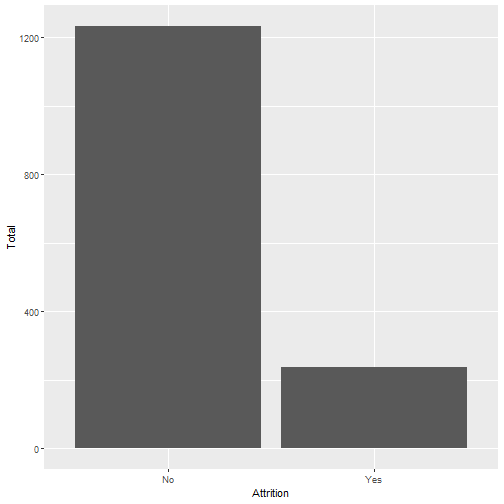
\includegraphics{IBM-HR-Analytics-ML-Classification_files/figure-latex/unnamed-chunk-8-1.pdf}

We also want to see the distribution of our employee's age divided by
their gender.

\begin{Shaded}
\begin{Highlighting}[]
\NormalTok{mean_age <-}\StringTok{ }\NormalTok{dataHR }\OperatorTok
\StringTok{    }\KeywordTok{group_by}\NormalTok{(Gender) }\OperatorTok
\StringTok{    }\KeywordTok{summarise}\NormalTok{(}\DataTypeTok{mean =} \KeywordTok{mean}\NormalTok{(Age),}
              \DataTypeTok{median =} \KeywordTok{median}\NormalTok{(Age)) }\OperatorTok
\StringTok{    }\KeywordTok{print}\NormalTok{()}
\end{Highlighting}
\end{Shaded}

\begin{verbatim}
## # A tibble: 2 x 3
##   Gender  mean median
##   <fct>  <dbl>  <dbl>
## 1 Female  37.3     36
## 2 Male    36.7     35
\end{verbatim}

\begin{Shaded}
\begin{Highlighting}[]
\NormalTok{plot1 <-}\StringTok{ }\NormalTok{dataHR }\OperatorTok\StringTok{ }
\StringTok{    }\KeywordTok{ggplot}\NormalTok{(}\KeywordTok{aes}\NormalTok{(}\DataTypeTok{x=}\NormalTok{Age)) }\OperatorTok{+}\StringTok{ }
\StringTok{    }\KeywordTok{geom_density}\NormalTok{(}\DataTypeTok{fill =} \StringTok{"green"}\NormalTok{, }\DataTypeTok{alpha =} \FloatTok{0.5}\NormalTok{) }\OperatorTok{+}
\StringTok{    }\KeywordTok{geom_vline}\NormalTok{(}\KeywordTok{aes}\NormalTok{(}\DataTypeTok{xintercept =} \KeywordTok{mean}\NormalTok{(Age)))}

\NormalTok{plot2 <-}\StringTok{ }\NormalTok{dataHR }\OperatorTok
\StringTok{    }\KeywordTok{filter}\NormalTok{(Gender }\OperatorTok{==}\StringTok{ "Male"}\NormalTok{) }\OperatorTok
\StringTok{    }\KeywordTok{ggplot}\NormalTok{(}\KeywordTok{aes}\NormalTok{(}\DataTypeTok{x=}\NormalTok{Age)) }\OperatorTok{+}\StringTok{ }
\StringTok{    }\KeywordTok{geom_density}\NormalTok{(}\DataTypeTok{fill =} \StringTok{"blue"}\NormalTok{, }\DataTypeTok{alpha =} \FloatTok{0.5}\NormalTok{) }\OperatorTok{+}
\StringTok{    }\KeywordTok{geom_vline}\NormalTok{(}\KeywordTok{aes}\NormalTok{(}\DataTypeTok{xintercept =} \KeywordTok{mean}\NormalTok{(Age)))}

\NormalTok{plot3 <-}\StringTok{ }\NormalTok{dataHR }\OperatorTok
\StringTok{    }\KeywordTok{filter}\NormalTok{(Gender }\OperatorTok{==}\StringTok{ "Female"}\NormalTok{) }\OperatorTok
\StringTok{    }\KeywordTok{ggplot}\NormalTok{(}\KeywordTok{aes}\NormalTok{(}\DataTypeTok{x=}\NormalTok{Age)) }\OperatorTok{+}\StringTok{ }
\StringTok{    }\KeywordTok{geom_density}\NormalTok{(}\DataTypeTok{fill =} \StringTok{"red"}\NormalTok{, }\DataTypeTok{alpha =} \FloatTok{0.5}\NormalTok{) }\OperatorTok{+}
\StringTok{    }\KeywordTok{geom_vline}\NormalTok{(}\KeywordTok{aes}\NormalTok{(}\DataTypeTok{xintercept =} \KeywordTok{mean}\NormalTok{(Age)))}

\KeywordTok{ggarrange}\NormalTok{(plot1,}
          \KeywordTok{ggarrange}\NormalTok{(plot2, plot3),}
          \DataTypeTok{nrow =} \DecValTok{2}\NormalTok{)}
\end{Highlighting}
\end{Shaded}

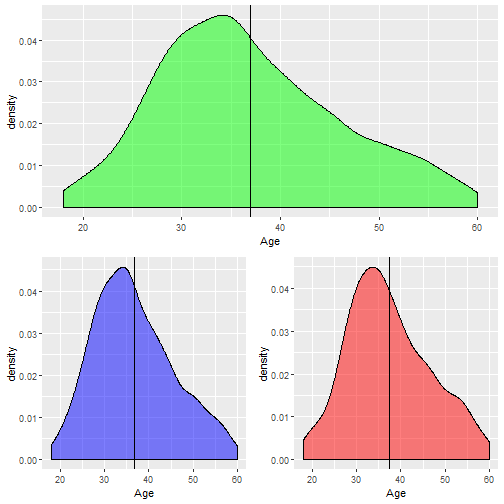
\includegraphics{IBM-HR-Analytics-ML-Classification_files/figure-latex/unnamed-chunk-10-1.pdf}

\begin{Shaded}
\begin{Highlighting}[]
\NormalTok{dist_attr_gender <-}\StringTok{ }\NormalTok{dataHR }\OperatorTok
\StringTok{                }\KeywordTok{group_by}\NormalTok{(Attrition, Gender) }\OperatorTok
\StringTok{                }\KeywordTok{summarise}\NormalTok{(}\DataTypeTok{Total =} \KeywordTok{n}\NormalTok{())}
\KeywordTok{print}\NormalTok{(dist_attr_gender)}
\end{Highlighting}
\end{Shaded}

\begin{verbatim}
## # A tibble: 4 x 3
## # Groups:   Attrition [2]
##   Attrition Gender Total
##   <fct>     <fct>  <int>
## 1 No        Female   501
## 2 No        Male     732
## 3 Yes       Female    87
## 4 Yes       Male     150
\end{verbatim}

\begin{Shaded}
\begin{Highlighting}[]
\NormalTok{dist_attr_gender }\OperatorTok
\StringTok{  }\KeywordTok{ggplot}\NormalTok{(}\KeywordTok{aes}\NormalTok{(}\DataTypeTok{x=}\NormalTok{Attrition, }\DataTypeTok{y=}\NormalTok{Total, }\DataTypeTok{fill=}\NormalTok{Gender)) }\OperatorTok{+}
\StringTok{  }\KeywordTok{geom_col}\NormalTok{(}\DataTypeTok{position=}\StringTok{"dodge"}\NormalTok{)}
\end{Highlighting}
\end{Shaded}

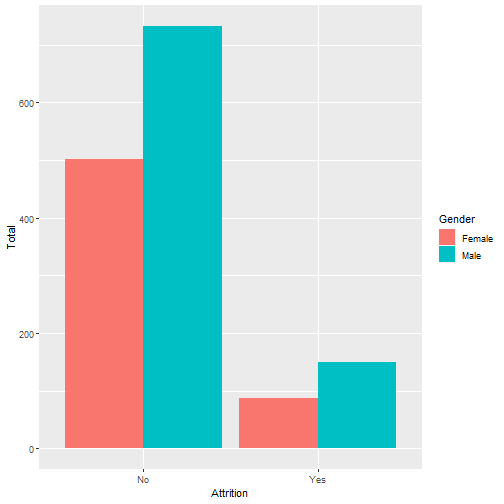
\includegraphics{IBM-HR-Analytics-ML-Classification_files/figure-latex/unnamed-chunk-12-1.pdf}

\begin{Shaded}
\begin{Highlighting}[]
\NormalTok{pie_attr_male <-}\StringTok{ }\NormalTok{dist_attr_gender }\OperatorTok
\StringTok{                    }\KeywordTok{filter}\NormalTok{(Gender }\OperatorTok{==}\StringTok{ "Male"}\NormalTok{) }\OperatorTok
\StringTok{                    }\KeywordTok{ggplot}\NormalTok{(}\KeywordTok{aes}\NormalTok{(}\DataTypeTok{x=}\StringTok{""}\NormalTok{, }\DataTypeTok{y=}\NormalTok{Total, }\DataTypeTok{fill=}\NormalTok{Attrition)) }\OperatorTok{+}
\StringTok{                    }\KeywordTok{geom_bar}\NormalTok{(}\DataTypeTok{width=}\DecValTok{1}\NormalTok{, }\DataTypeTok{stat=}\StringTok{"identity"}\NormalTok{) }\OperatorTok{+}\StringTok{ }
\StringTok{                    }\KeywordTok{coord_polar}\NormalTok{(}\StringTok{"y"}\NormalTok{, }\DataTypeTok{start=}\DecValTok{0}\NormalTok{) }\OperatorTok{+}
\StringTok{                    }\KeywordTok{ggtitle}\NormalTok{(}\StringTok{"Pie Chart }\CharTok{\textbackslash{}n}\StringTok{Attrition Male"}\NormalTok{) }\OperatorTok{+}
\StringTok{                    }\KeywordTok{geom_text}\NormalTok{(}\KeywordTok{aes}\NormalTok{(}\DataTypeTok{y =}\NormalTok{ Total}\OperatorTok{/}\DecValTok{2} \OperatorTok{+}\StringTok{ }\KeywordTok{c}\NormalTok{(}\DecValTok{5}\NormalTok{, }\DecValTok{10}\NormalTok{), }
                              \DataTypeTok{label =} \KeywordTok{percent}\NormalTok{(Total}\OperatorTok{/}\KeywordTok{sum}\NormalTok{(Total))), }\DataTypeTok{size=}\DecValTok{5}\NormalTok{)}

\NormalTok{pie_attr_female <-}\StringTok{ }\NormalTok{dist_attr_gender }\OperatorTok
\StringTok{                    }\KeywordTok{filter}\NormalTok{(Gender }\OperatorTok{==}\StringTok{ "Female"}\NormalTok{) }\OperatorTok
\StringTok{                    }\KeywordTok{ggplot}\NormalTok{(}\KeywordTok{aes}\NormalTok{(}\DataTypeTok{x=}\StringTok{""}\NormalTok{, }\DataTypeTok{y=}\NormalTok{Total, }\DataTypeTok{fill=}\NormalTok{Attrition)) }\OperatorTok{+}
\StringTok{                    }\KeywordTok{geom_bar}\NormalTok{(}\DataTypeTok{width=}\DecValTok{1}\NormalTok{, }\DataTypeTok{stat=}\StringTok{"identity"}\NormalTok{) }\OperatorTok{+}\StringTok{ }
\StringTok{                    }\KeywordTok{coord_polar}\NormalTok{(}\StringTok{"y"}\NormalTok{, }\DataTypeTok{start=}\DecValTok{0}\NormalTok{) }\OperatorTok{+}
\StringTok{                    }\KeywordTok{ggtitle}\NormalTok{(}\StringTok{"Pie Chart }\CharTok{\textbackslash{}n}\StringTok{Attrition Female"}\NormalTok{) }\OperatorTok{+}
\StringTok{                    }\KeywordTok{geom_text}\NormalTok{(}\KeywordTok{aes}\NormalTok{(}\DataTypeTok{y =}\NormalTok{ Total}\OperatorTok{/}\DecValTok{2} \OperatorTok{+}\StringTok{ }\KeywordTok{c}\NormalTok{(}\DecValTok{5}\NormalTok{, }\DecValTok{10}\NormalTok{), }
                              \DataTypeTok{label =} \KeywordTok{percent}\NormalTok{(Total}\OperatorTok{/}\KeywordTok{sum}\NormalTok{(Total))), }\DataTypeTok{size=}\DecValTok{5}\NormalTok{)}

\KeywordTok{ggarrange}\NormalTok{(pie_attr_male, pie_attr_female)}
\end{Highlighting}
\end{Shaded}

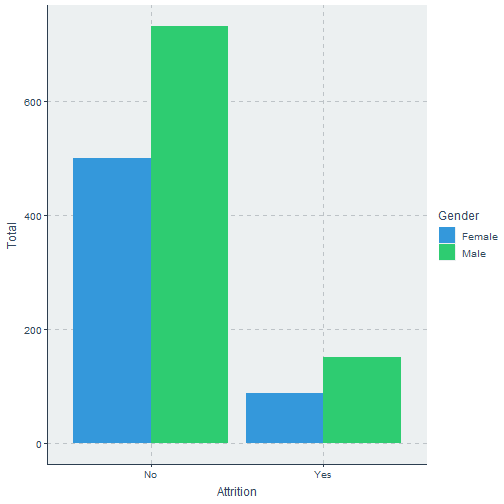
\includegraphics{IBM-HR-Analytics-ML-Classification_files/figure-latex/unnamed-chunk-13-1.pdf}

\hypertarget{modelling}{%
\section{Modelling}\label{modelling}}

\hypertarget{logistic-regression}{%
\subsection{Logistic Regression}\label{logistic-regression}}

Our variable of interest is the \textbf{Attrition} variable that
indicate whether the employee considered in the Attrition group
(Attrition = Yes) or the opposite (Attrition = No).

\begin{Shaded}
\begin{Highlighting}[]
\KeywordTok{head}\NormalTok{(dataHR}\OperatorTok{$}\NormalTok{Attrition)}
\end{Highlighting}
\end{Shaded}

\begin{verbatim}
## [1] Yes No  Yes No  No  No 
## Levels: No Yes
\end{verbatim}

We will divide our dataset into 80\% in train data and 20\% in test
data. We will using set.seed() function to make sure that R produce the
same random number to make this report is reproducible.

\begin{Shaded}
\begin{Highlighting}[]
\KeywordTok{RNGkind}\NormalTok{(}\DataTypeTok{sample.kind =} \StringTok{"Rounding"}\NormalTok{)}
\end{Highlighting}
\end{Shaded}

\begin{verbatim}
## Warning in RNGkind(sample.kind = "Rounding"): non-uniform 'Rounding' sampler
## used
\end{verbatim}

\begin{Shaded}
\begin{Highlighting}[]
\KeywordTok{set.seed}\NormalTok{(}\DecValTok{18}\NormalTok{)}
\NormalTok{index <-}\StringTok{ }\KeywordTok{sample}\NormalTok{(}\KeywordTok{nrow}\NormalTok{(dataHR), }\KeywordTok{nrow}\NormalTok{(dataHR)}\OperatorTok{*}\FloatTok{0.8}\NormalTok{)}
\NormalTok{data_train <-}\StringTok{ }\NormalTok{dataHR[index, ]}
\NormalTok{data_test <-}\StringTok{ }\NormalTok{dataHR[}\OperatorTok{-}\NormalTok{index,]}
\end{Highlighting}
\end{Shaded}

Before doing any analysis, we must make sure that we have a balanced
training data. An imbalanced training data most likely to perform poorer
that the balanced data. So, we will try to make it balanced by using an
upsampling technique with ovun.sample() function from ROSE package.

We will see our train data distribution.

\begin{Shaded}
\begin{Highlighting}[]
\KeywordTok{table}\NormalTok{(data_train}\OperatorTok{$}\NormalTok{Attrition)}
\end{Highlighting}
\end{Shaded}

\begin{verbatim}
## 
##  No Yes 
## 996 180
\end{verbatim}

Upsampling the data and see again the train data distribution.

\begin{Shaded}
\begin{Highlighting}[]
\NormalTok{train_balanced <-}\StringTok{ }\KeywordTok{ovun.sample}\NormalTok{(Attrition }\OperatorTok{~}\StringTok{ }\NormalTok{., }\DataTypeTok{data =}\NormalTok{ data_train, }\DataTypeTok{method =} \StringTok{"over"}\NormalTok{,}
                              \DataTypeTok{N =} \DecValTok{996}\OperatorTok{*}\DecValTok{2}\NormalTok{, }\DataTypeTok{seed =} \DecValTok{1}\NormalTok{)}\OperatorTok{$}\NormalTok{data}
\KeywordTok{table}\NormalTok{(train_balanced}\OperatorTok{$}\NormalTok{Attrition)}
\end{Highlighting}
\end{Shaded}

\begin{verbatim}
## 
##  No Yes 
## 996 996
\end{verbatim}

After the data is balanced, we will make out first Logistic Regression
model by using all the predictors into the formula.

\begin{Shaded}
\begin{Highlighting}[]
\NormalTok{model_log_full <-}\StringTok{ }\KeywordTok{glm}\NormalTok{(Attrition }\OperatorTok{~}\StringTok{ }\NormalTok{., }\DataTypeTok{family =} \StringTok{"binomial"}\NormalTok{, }\DataTypeTok{data =}\NormalTok{ train_balanced)}
\KeywordTok{summary}\NormalTok{(model_log_full)}
\end{Highlighting}
\end{Shaded}

\begin{verbatim}
## 
## Call:
## glm(formula = Attrition ~ ., family = "binomial", data = train_balanced)
## 
## Deviance Residuals: 
##     Min       1Q   Median       3Q      Max  
## -2.8672  -0.5173   0.0246   0.5847   3.4560  
## 
## Coefficients:
##                                    Estimate Std. Error z value Pr(>|z|)    
## (Intercept)                      -9.801e+00  3.256e+02  -0.030 0.975983    
## Age                              -3.858e-02  1.031e-02  -3.741 0.000183 ***
## BusinessTravelTravel_Frequently   2.260e+00  3.203e-01   7.054 1.74e-12 ***
## BusinessTravelTravel_Rarely       1.224e+00  2.896e-01   4.226 2.38e-05 ***
## DailyRate                        -4.255e-04  1.751e-04  -2.429 0.015120 *  
## DepartmentResearch & Development  1.521e+01  3.256e+02   0.047 0.962735    
## DepartmentSales                   1.505e+01  3.256e+02   0.046 0.963137    
## DistanceFromHome                  4.566e-02  8.898e-03   5.132 2.87e-07 ***
## Education2                       -1.167e-02  2.495e-01  -0.047 0.962693    
## Education3                       -9.487e-02  2.207e-01  -0.430 0.667304    
## Education4                        2.541e-01  2.422e-01   1.049 0.294043    
## Education5                        2.890e-01  4.320e-01   0.669 0.503559    
## EducationFieldLife Sciences      -1.471e+00  6.599e-01  -2.229 0.025842 *  
## EducationFieldMarketing          -6.816e-01  6.877e-01  -0.991 0.321555    
## EducationFieldMedical            -1.346e+00  6.509e-01  -2.068 0.038676 *  
## EducationFieldOther              -8.496e-01  6.986e-01  -1.216 0.223902    
## EducationFieldTechnical Degree    1.691e-01  6.741e-01   0.251 0.801992    
## EmployeeNumber                   -2.245e-04  1.224e-04  -1.834 0.066652 .  
## EnvironmentSatisfaction2         -1.244e+00  2.258e-01  -5.509 3.60e-08 ***
## EnvironmentSatisfaction3         -1.090e+00  2.059e-01  -5.296 1.18e-07 ***
## EnvironmentSatisfaction4         -1.111e+00  2.029e-01  -5.473 4.41e-08 ***
## GenderMale                        4.716e-01  1.448e-01   3.258 0.001124 ** 
## HourlyRate                       -1.655e-03  3.419e-03  -0.484 0.628366    
## JobInvolvement2                  -1.240e+00  3.224e-01  -3.846 0.000120 ***
## JobInvolvement3                  -1.580e+00  3.078e-01  -5.133 2.85e-07 ***
## JobInvolvement4                  -1.678e+00  3.808e-01  -4.408 1.05e-05 ***
## JobLevel2                        -1.025e+00  2.986e-01  -3.433 0.000596 ***
## JobLevel3                         1.023e+00  5.256e-01   1.946 0.051666 .  
## JobLevel4                        -2.091e+00  9.785e-01  -2.137 0.032572 *  
## JobLevel5                         3.386e+00  1.189e+00   2.848 0.004400 ** 
## JobRoleHuman Resources            1.642e+01  3.256e+02   0.050 0.959764    
## JobRoleLaboratory Technician      2.041e+00  4.764e-01   4.284 1.83e-05 ***
## JobRoleManager                   -3.228e-01  8.494e-01  -0.380 0.703927    
## JobRoleManufacturing Director     1.068e+00  4.715e-01   2.264 0.023555 *  
## JobRoleResearch Director         -2.529e+00  9.117e-01  -2.774 0.005531 ** 
## JobRoleResearch Scientist         1.107e+00  4.789e-01   2.312 0.020776 *  
## JobRoleSales Executive            2.459e+00  1.007e+00   2.442 0.014620 *  
## JobRoleSales Representative       3.035e+00  1.061e+00   2.862 0.004213 ** 
## JobSatisfaction2                 -1.168e+00  2.168e-01  -5.387 7.17e-08 ***
## JobSatisfaction3                 -8.921e-01  1.891e-01  -4.718 2.38e-06 ***
## JobSatisfaction4                 -1.750e+00  2.043e-01  -8.564  < 2e-16 ***
## MaritalStatusMarried              5.933e-01  2.022e-01   2.935 0.003338 ** 
## MaritalStatusSingle               6.732e-01  2.930e-01   2.297 0.021591 *  
## MonthlyIncome                    -1.466e-04  7.005e-05  -2.093 0.036321 *  
## MonthlyRate                       9.625e-06  9.522e-06   1.011 0.312118    
## NumCompaniesWorked                2.380e-01  3.096e-02   7.687 1.50e-14 ***
## OverTimeYes                       2.020e+00  1.534e-01  13.166  < 2e-16 ***
## PercentSalaryHike                -6.368e-02  3.011e-02  -2.115 0.034450 *  
## PerformanceRating4                2.976e-01  3.191e-01   0.933 0.351078    
## RelationshipSatisfaction2        -1.149e+00  2.183e-01  -5.264 1.41e-07 ***
## RelationshipSatisfaction3        -1.045e+00  1.955e-01  -5.347 8.93e-08 ***
## RelationshipSatisfaction4        -1.094e+00  1.970e-01  -5.552 2.82e-08 ***
## StockOptionLevel1                -1.274e+00  2.405e-01  -5.299 1.16e-07 ***
## StockOptionLevel2                -1.131e+00  3.153e-01  -3.586 0.000336 ***
## StockOptionLevel3                -3.910e-01  3.662e-01  -1.068 0.285618    
## TotalWorkingYears                -3.083e-02  2.078e-02  -1.483 0.138032    
## TrainingTimesLastYear            -1.209e-01  5.217e-02  -2.318 0.020468 *  
## WorkLifeBalance2                 -9.685e-01  2.946e-01  -3.288 0.001008 ** 
## WorkLifeBalance3                 -1.549e+00  2.815e-01  -5.503 3.73e-08 ***
## WorkLifeBalance4                 -6.003e-01  3.325e-01  -1.805 0.071037 .  
## YearsAtCompany                    2.011e-01  3.016e-02   6.670 2.56e-11 ***
## YearsInCurrentRole               -2.519e-01  4.021e-02  -6.266 3.70e-10 ***
## YearsSinceLastPromotion           1.024e-01  3.173e-02   3.225 0.001258 ** 
## YearsWithCurrManager             -1.281e-01  3.721e-02  -3.444 0.000573 ***
## ---
## Signif. codes:  0 '***' 0.001 '**' 0.01 '*' 0.05 '.' 0.1 ' ' 1
## 
## (Dispersion parameter for binomial family taken to be 1)
## 
##     Null deviance: 2761.5  on 1991  degrees of freedom
## Residual deviance: 1511.3  on 1928  degrees of freedom
## AIC: 1639.3
## 
## Number of Fisher Scoring iterations: 14
\end{verbatim}

We will detect if perfect separation exist in our data.
\url{https://cran.r-project.org/web/packages/brglm2/vignettes/separation.html}

\begin{Shaded}
\begin{Highlighting}[]
\KeywordTok{glm}\NormalTok{(}\DataTypeTok{formula =}\NormalTok{ Attrition }\OperatorTok{~}\StringTok{ }\NormalTok{., }\DataTypeTok{family =} \StringTok{"binomial"}\NormalTok{, }\DataTypeTok{data =}\NormalTok{ data_train, }\DataTypeTok{method =} \StringTok{"detect_separation"}\NormalTok{, }\DataTypeTok{linear_program =} \StringTok{"dual"}\NormalTok{)}
\end{Highlighting}
\end{Shaded}

\begin{verbatim}
## Separation: FALSE 
## Existence of maximum likelihood estimates
##                      (Intercept)                              Age 
##                             -Inf                                0 
##  BusinessTravelTravel_Frequently      BusinessTravelTravel_Rarely 
##                                0                                0 
##                        DailyRate DepartmentResearch & Development 
##                                0                              Inf 
##                  DepartmentSales                 DistanceFromHome 
##                              Inf                                0 
##                       Education2                       Education3 
##                                0                                0 
##                       Education4                       Education5 
##                                0                                0 
##      EducationFieldLife Sciences          EducationFieldMarketing 
##                                0                                0 
##            EducationFieldMedical              EducationFieldOther 
##                                0                                0 
##   EducationFieldTechnical Degree                   EmployeeNumber 
##                                0                                0 
##         EnvironmentSatisfaction2         EnvironmentSatisfaction3 
##                                0                                0 
##         EnvironmentSatisfaction4                       GenderMale 
##                                0                                0 
##                       HourlyRate                  JobInvolvement2 
##                                0                                0 
##                  JobInvolvement3                  JobInvolvement4 
##                                0                                0 
##                        JobLevel2                        JobLevel3 
##                                0                                0 
##                        JobLevel4                        JobLevel5 
##                                0                                0 
##           JobRoleHuman Resources     JobRoleLaboratory Technician 
##                              Inf                                0 
##                   JobRoleManager    JobRoleManufacturing Director 
##                                0                                0 
##         JobRoleResearch Director        JobRoleResearch Scientist 
##                                0                                0 
##           JobRoleSales Executive      JobRoleSales Representative 
##                                0                                0 
##                 JobSatisfaction2                 JobSatisfaction3 
##                                0                                0 
##                 JobSatisfaction4             MaritalStatusMarried 
##                                0                                0 
##              MaritalStatusSingle                    MonthlyIncome 
##                                0                                0 
##                      MonthlyRate               NumCompaniesWorked 
##                                0                                0 
##                      OverTimeYes                PercentSalaryHike 
##                                0                                0 
##               PerformanceRating4        RelationshipSatisfaction2 
##                                0                                0 
##        RelationshipSatisfaction3        RelationshipSatisfaction4 
##                                0                                0 
##                StockOptionLevel1                StockOptionLevel2 
##                                0                                0 
##                StockOptionLevel3                TotalWorkingYears 
##                                0                                0 
##            TrainingTimesLastYear                 WorkLifeBalance2 
##                                0                                0 
##                 WorkLifeBalance3                 WorkLifeBalance4 
##                                0                                0 
##                   YearsAtCompany               YearsInCurrentRole 
##                                0                                0 
##          YearsSinceLastPromotion             YearsWithCurrManager 
##                                0                                0 
## 0: finite value, Inf: infinity, -Inf: -infinity
\end{verbatim}

We will doing a feature engineering by applying the step() function into
our full model. We will using the backward option, which the function
will iterate over the model, starts with all predictor (full model as we
input it) and remove the least contributive predictors.

\begin{Shaded}
\begin{Highlighting}[]
\NormalTok{model_log_bw <-}\StringTok{ }\KeywordTok{step}\NormalTok{(model_log_full, }\DataTypeTok{direction =} \StringTok{"backward"}\NormalTok{, }\DataTypeTok{trace =} \OtherTok{FALSE}\NormalTok{)}
\KeywordTok{summary}\NormalTok{(model_log_bw)}
\end{Highlighting}
\end{Shaded}

\begin{verbatim}
## 
## Call:
## glm(formula = Attrition ~ Age + BusinessTravel + DailyRate + 
##     Department + DistanceFromHome + EducationField + EmployeeNumber + 
##     EnvironmentSatisfaction + Gender + JobInvolvement + JobLevel + 
##     JobRole + JobSatisfaction + MaritalStatus + MonthlyIncome + 
##     NumCompaniesWorked + OverTime + PercentSalaryHike + RelationshipSatisfaction + 
##     StockOptionLevel + TotalWorkingYears + TrainingTimesLastYear + 
##     WorkLifeBalance + YearsAtCompany + YearsInCurrentRole + YearsSinceLastPromotion + 
##     YearsWithCurrManager, family = "binomial", data = train_balanced)
## 
## Deviance Residuals: 
##     Min       1Q   Median       3Q      Max  
## -2.8611  -0.5238   0.0286   0.5907   3.4512  
## 
## Coefficients:
##                                    Estimate Std. Error z value Pr(>|z|)    
## (Intercept)                      -1.020e+01  3.216e+02  -0.032 0.974706    
## Age                              -3.617e-02  1.003e-02  -3.607 0.000310 ***
## BusinessTravelTravel_Frequently   2.247e+00  3.185e-01   7.054 1.73e-12 ***
## BusinessTravelTravel_Rarely       1.235e+00  2.873e-01   4.298 1.72e-05 ***
## DailyRate                        -4.102e-04  1.721e-04  -2.384 0.017135 *  
## DepartmentResearch & Development  1.535e+01  3.216e+02   0.048 0.961932    
## DepartmentSales                   1.518e+01  3.216e+02   0.047 0.962360    
## DistanceFromHome                  4.663e-02  8.788e-03   5.307 1.12e-07 ***
## EducationFieldLife Sciences      -1.530e+00  6.345e-01  -2.411 0.015903 *  
## EducationFieldMarketing          -7.559e-01  6.685e-01  -1.131 0.258195    
## EducationFieldMedical            -1.436e+00  6.248e-01  -2.299 0.021518 *  
## EducationFieldOther              -8.717e-01  6.693e-01  -1.302 0.192746    
## EducationFieldTechnical Degree    4.438e-02  6.511e-01   0.068 0.945657    
## EmployeeNumber                   -2.060e-04  1.209e-04  -1.703 0.088483 .  
## EnvironmentSatisfaction2         -1.228e+00  2.241e-01  -5.481 4.22e-08 ***
## EnvironmentSatisfaction3         -1.073e+00  2.041e-01  -5.257 1.47e-07 ***
## EnvironmentSatisfaction4         -1.081e+00  2.009e-01  -5.381 7.42e-08 ***
## GenderMale                        4.882e-01  1.436e-01   3.400 0.000673 ***
## JobInvolvement2                  -1.221e+00  3.185e-01  -3.832 0.000127 ***
## JobInvolvement3                  -1.556e+00  3.013e-01  -5.163 2.44e-07 ***
## JobInvolvement4                  -1.678e+00  3.747e-01  -4.478 7.54e-06 ***
## JobLevel2                        -1.005e+00  2.963e-01  -3.390 0.000698 ***
## JobLevel3                         1.020e+00  5.201e-01   1.961 0.049846 *  
## JobLevel4                        -2.127e+00  9.762e-01  -2.179 0.029357 *  
## JobLevel5                         3.288e+00  1.176e+00   2.796 0.005179 ** 
## JobRoleHuman Resources            1.645e+01  3.216e+02   0.051 0.959207    
## JobRoleLaboratory Technician      1.983e+00  4.728e-01   4.195 2.73e-05 ***
## JobRoleManager                   -1.912e-01  8.395e-01  -0.228 0.819847    
## JobRoleManufacturing Director     1.051e+00  4.682e-01   2.245 0.024773 *  
## JobRoleResearch Director         -2.265e+00  8.983e-01  -2.522 0.011679 *  
## JobRoleResearch Scientist         1.058e+00  4.758e-01   2.224 0.026168 *  
## JobRoleSales Executive            2.461e+00  1.011e+00   2.434 0.014931 *  
## JobRoleSales Representative       2.974e+00  1.065e+00   2.794 0.005207 ** 
## JobSatisfaction2                 -1.168e+00  2.138e-01  -5.463 4.68e-08 ***
## JobSatisfaction3                 -8.703e-01  1.861e-01  -4.677 2.92e-06 ***
## JobSatisfaction4                 -1.731e+00  2.005e-01  -8.635  < 2e-16 ***
## MaritalStatusMarried              5.959e-01  1.996e-01   2.986 0.002826 ** 
## MaritalStatusSingle               6.371e-01  2.893e-01   2.203 0.027626 *  
## MonthlyIncome                    -1.574e-04  6.925e-05  -2.272 0.023069 *  
## NumCompaniesWorked                2.340e-01  3.066e-02   7.632 2.31e-14 ***
## OverTimeYes                       2.012e+00  1.516e-01  13.270  < 2e-16 ***
## PercentSalaryHike                -4.092e-02  1.929e-02  -2.121 0.033902 *  
## RelationshipSatisfaction2        -1.112e+00  2.130e-01  -5.222 1.77e-07 ***
## RelationshipSatisfaction3        -1.010e+00  1.918e-01  -5.267 1.39e-07 ***
## RelationshipSatisfaction4        -1.046e+00  1.948e-01  -5.371 7.83e-08 ***
## StockOptionLevel1                -1.356e+00  2.350e-01  -5.771 7.87e-09 ***
## StockOptionLevel2                -1.197e+00  3.086e-01  -3.879 0.000105 ***
## StockOptionLevel3                -4.014e-01  3.607e-01  -1.113 0.265790    
## TotalWorkingYears                -2.977e-02  2.054e-02  -1.449 0.147289    
## TrainingTimesLastYear            -1.282e-01  5.158e-02  -2.486 0.012915 *  
## WorkLifeBalance2                 -9.798e-01  2.906e-01  -3.372 0.000745 ***
## WorkLifeBalance3                 -1.531e+00  2.757e-01  -5.553 2.81e-08 ***
## WorkLifeBalance4                 -6.113e-01  3.278e-01  -1.865 0.062216 .  
## YearsAtCompany                    2.056e-01  3.004e-02   6.845 7.65e-12 ***
## YearsInCurrentRole               -2.527e-01  4.009e-02  -6.303 2.92e-10 ***
## YearsSinceLastPromotion           1.046e-01  3.127e-02   3.345 0.000824 ***
## YearsWithCurrManager             -1.277e-01  3.683e-02  -3.466 0.000528 ***
## ---
## Signif. codes:  0 '***' 0.001 '**' 0.01 '*' 0.05 '.' 0.1 ' ' 1
## 
## (Dispersion parameter for binomial family taken to be 1)
## 
##     Null deviance: 2761.5  on 1991  degrees of freedom
## Residual deviance: 1517.1  on 1935  degrees of freedom
## AIC: 1631.1
## 
## Number of Fisher Scoring iterations: 14
\end{verbatim}

No we will check if multicollinearity exist in our model using vif()
function from car package. According to Zuur et al.~(2010), a high value
of VIF indicating a multicollinearity exist and suggest to drop the
highest value of VIF.

\begin{Shaded}
\begin{Highlighting}[]
\NormalTok{car}\OperatorTok{::}\KeywordTok{vif}\NormalTok{(model_log_bw)}
\end{Highlighting}
\end{Shaded}

\begin{verbatim}
##                                  GVIF Df GVIF^(1/(2*Df))
## Age                      1.987430e+00  1        1.409763
## BusinessTravel           1.338507e+00  2        1.075611
## DailyRate                1.175317e+00  1        1.084120
## Department               5.743169e+07  2       87.053832
## DistanceFromHome         1.228154e+00  1        1.108221
## EducationField           4.666025e+00  5        1.166527
## EmployeeNumber           1.185489e+00  1        1.088801
## EnvironmentSatisfaction  1.636246e+00  3        1.085529
## Gender                   1.147067e+00  1        1.071012
## JobInvolvement           1.598506e+00  3        1.081315
## JobLevel                 7.672646e+01  4        1.720355
## JobRole                  1.243779e+09  8        3.701873
## JobSatisfaction          1.595519e+00  3        1.080978
## MaritalStatus            3.569071e+00  2        1.374481
## MonthlyIncome            1.533085e+01  1        3.915463
## NumCompaniesWorked       1.523547e+00  1        1.234321
## OverTime                 1.308205e+00  1        1.143768
## PercentSalaryHike        1.128670e+00  1        1.062389
## RelationshipSatisfaction 1.508066e+00  3        1.070870
## StockOptionLevel         4.275539e+00  3        1.273987
## TotalWorkingYears        5.195686e+00  1        2.279405
## TrainingTimesLastYear    1.135342e+00  1        1.065524
## WorkLifeBalance          1.602410e+00  3        1.081755
## YearsAtCompany           7.559767e+00  1        2.749503
## YearsInCurrentRole       4.249090e+00  1        2.061332
## YearsSinceLastPromotion  2.307515e+00  1        1.519051
## YearsWithCurrManager     3.736256e+00  1        1.932940
\end{verbatim}

Recreating a formula with the highest VIF is dropped.

\begin{Shaded}
\begin{Highlighting}[]
\NormalTok{model_log_bw <-}\StringTok{ }\KeywordTok{glm}\NormalTok{(}\DataTypeTok{formula =}\NormalTok{ Attrition }\OperatorTok{~}\StringTok{ }\NormalTok{Age }\OperatorTok{+}\StringTok{ }\NormalTok{BusinessTravel }\OperatorTok{+}\StringTok{ }\NormalTok{DailyRate }\OperatorTok{+}\StringTok{ }
\StringTok{    }\NormalTok{DistanceFromHome }\OperatorTok{+}\StringTok{ }\NormalTok{EducationField }\OperatorTok{+}\StringTok{ }\NormalTok{EmployeeNumber }\OperatorTok{+}\StringTok{ }
\StringTok{    }\NormalTok{EnvironmentSatisfaction }\OperatorTok{+}\StringTok{ }\NormalTok{Gender }\OperatorTok{+}\StringTok{ }\NormalTok{JobInvolvement }\OperatorTok{+}\StringTok{ }\NormalTok{JobLevel }\OperatorTok{+}\StringTok{ }
\StringTok{    }\NormalTok{JobRole }\OperatorTok{+}\StringTok{ }\NormalTok{JobSatisfaction }\OperatorTok{+}\StringTok{ }\NormalTok{MaritalStatus }\OperatorTok{+}\StringTok{ }\NormalTok{MonthlyIncome }\OperatorTok{+}\StringTok{ }
\StringTok{    }\NormalTok{NumCompaniesWorked }\OperatorTok{+}\StringTok{ }\NormalTok{OverTime }\OperatorTok{+}\StringTok{ }\NormalTok{PercentSalaryHike }\OperatorTok{+}\StringTok{ }\NormalTok{RelationshipSatisfaction }\OperatorTok{+}\StringTok{ }
\StringTok{    }\NormalTok{StockOptionLevel }\OperatorTok{+}\StringTok{ }\NormalTok{TotalWorkingYears }\OperatorTok{+}\StringTok{ }\NormalTok{TrainingTimesLastYear }\OperatorTok{+}\StringTok{ }
\StringTok{    }\NormalTok{WorkLifeBalance }\OperatorTok{+}\StringTok{ }\NormalTok{YearsAtCompany }\OperatorTok{+}\StringTok{ }\NormalTok{YearsInCurrentRole }\OperatorTok{+}\StringTok{ }\NormalTok{YearsSinceLastPromotion }\OperatorTok{+}\StringTok{ }
\StringTok{    }\NormalTok{YearsWithCurrManager, }\DataTypeTok{family =} \StringTok{"binomial"}\NormalTok{, }\DataTypeTok{data =}\NormalTok{ train_balanced)}
\end{Highlighting}
\end{Shaded}

Recalculate the VIF value.

\begin{Shaded}
\begin{Highlighting}[]
\NormalTok{car}\OperatorTok{::}\KeywordTok{vif}\NormalTok{(model_log_bw)}
\end{Highlighting}
\end{Shaded}

\begin{verbatim}
##                               GVIF Df GVIF^(1/(2*Df))
## Age                       1.983295  1        1.408295
## BusinessTravel            1.329186  2        1.073733
## DailyRate                 1.175157  1        1.084047
## DistanceFromHome          1.216231  1        1.102829
## EducationField            4.315324  5        1.157448
## EmployeeNumber            1.182660  1        1.087502
## EnvironmentSatisfaction   1.614912  3        1.083157
## Gender                    1.138396  1        1.066956
## JobInvolvement            1.549342  3        1.075700
## JobLevel                 73.886948  4        1.712265
## JobRole                  77.216664  8        1.312145
## JobSatisfaction           1.574728  3        1.078618
## MaritalStatus             3.560918  2        1.373696
## MonthlyIncome            15.480245  1        3.934494
## NumCompaniesWorked        1.516519  1        1.231470
## OverTime                  1.298094  1        1.139339
## PercentSalaryHike         1.124487  1        1.060418
## RelationshipSatisfaction  1.497423  3        1.069607
## StockOptionLevel          4.255169  3        1.272974
## TotalWorkingYears         5.173397  1        2.274510
## TrainingTimesLastYear     1.134146  1        1.064963
## WorkLifeBalance           1.598007  3        1.081259
## YearsAtCompany            7.271288  1        2.696533
## YearsInCurrentRole        4.092361  1        2.022959
## YearsSinceLastPromotion   2.249532  1        1.499844
## YearsWithCurrManager      3.700395  1        1.923641
\end{verbatim}

After the highest value of VIF dropped, our model is ready to be used
for predicting the test dataset.

\begin{Shaded}
\begin{Highlighting}[]
\NormalTok{pred <-}\StringTok{ }\KeywordTok{predict}\NormalTok{(model_log_bw, data_test, }\StringTok{"response"}\NormalTok{)}
\end{Highlighting}
\end{Shaded}

Let say the company objective is want to prevent the Attrition, so we
don´t want to predict the Attrition = No when it is actually Yes.

If the real value of Attrition = Yes while the predicted value is No, it
will make us failed to take a preventive action that needed to take to
prevent the Attrition is happened.

If the real value of Attrition = No while the predicted valus is Yes, we
may take an unnecessary step to prevent something that won't happened.
But in my opinion, this action is not fatal and maybe it better, because
with this `mistaken' step is taken, we may actually build a stronger
relationship and stronger understanding with our employee. Not a bad
choice actually.

FP: a test result which incorrectly indicates that a particular
condition or attribute is present. FN: a test result which incorrectly
indicates that a particular condition or attribute is absent.

So, in our case, we prefer to focus to lowering the \textbf{False
Negatives} rate. Why? Because if so, we will miss our valuable employee.

In the False Positive case, when the actual is good, we may take the
concrete step, like questioning our own employee. But in the end, we
will figure out that our employee have no problem at all.

Sensitivity = TP/(TP + FN) Specificity = TN/(TN + FP) Accuracy = (TN +
TP)/(TN+TP+FN+FP)

So, we want to \textbf{decrease} the FN. According to the formula, if we
decrease the FN, we will increase the Sensitivity and the Accuracy
score.

Now we will compare our prediction with the real value in the test
dataset. The threshold is set into 0.5.

\begin{Shaded}
\begin{Highlighting}[]
\NormalTok{pred_round <-}\StringTok{ }\KeywordTok{as.factor}\NormalTok{(}\KeywordTok{ifelse}\NormalTok{(pred }\OperatorTok{>=}\StringTok{ }\FloatTok{0.5}\NormalTok{, }\StringTok{"Yes"}\NormalTok{, }\StringTok{"No"}\NormalTok{))}
\KeywordTok{confusionMatrix}\NormalTok{(pred_round, data_test}\OperatorTok{$}\NormalTok{Attrition, }\DataTypeTok{positive =} \StringTok{"Yes"}\NormalTok{)}
\end{Highlighting}
\end{Shaded}

\begin{verbatim}
## Confusion Matrix and Statistics
## 
##           Reference
## Prediction  No Yes
##        No  186  13
##        Yes  51  44
##                                           
##                Accuracy : 0.7823          
##                  95% CI : (0.7307, 0.8281)
##     No Information Rate : 0.8061          
##     P-Value [Acc > NIR] : 0.8651          
##                                           
##                   Kappa : 0.4443          
##                                           
##  Mcnemar's Test P-Value : 3.746e-06       
##                                           
##             Sensitivity : 0.7719          
##             Specificity : 0.7848          
##          Pos Pred Value : 0.4632          
##          Neg Pred Value : 0.9347          
##              Prevalence : 0.1939          
##          Detection Rate : 0.1497          
##    Detection Prevalence : 0.3231          
##       Balanced Accuracy : 0.7784          
##                                           
##        'Positive' Class : Yes             
## 
\end{verbatim}

We will try to increase the accuracy and decrease the FN. In the
Logistic Regression model, it can happen by adjusting the threshold of
the prediction. But the question, what is the optimal number of the
threshold? We will create a graph that will help us visualize the
distribution of the prediction.

\begin{Shaded}
\begin{Highlighting}[]
\NormalTok{data_test}\OperatorTok{$}\NormalTok{pred <-}\StringTok{ }\NormalTok{pred}

\KeywordTok{ggplot}\NormalTok{(data_test, }\KeywordTok{aes}\NormalTok{(pred, }\DataTypeTok{color =} \KeywordTok{as.factor}\NormalTok{(Attrition) ) ) }\OperatorTok{+}\StringTok{ }
\KeywordTok{geom_density}\NormalTok{( }\DataTypeTok{size =} \DecValTok{1}\NormalTok{ ) }\OperatorTok{+}
\KeywordTok{ggtitle}\NormalTok{(}\StringTok{"Testing Set's Predicted Score"}\NormalTok{) }
\end{Highlighting}
\end{Shaded}

\includegraphics{IBM-HR-Analytics-ML-Classification_files/figure-latex/unnamed-chunk-26-1.pdf}

By seeing above graph, we can tuning our model by adjusting the
threshold: - The threshold value of \textless0.5 will results in more
Attrition == Yes - The threshold value of \textgreater0.5 will results
in less Attrition == Yes

Beside graph, we can mathematically compute the most optimal cutoff
values.

\begin{Shaded}
\begin{Highlighting}[]
\NormalTok{ROCRpred =}\StringTok{ }\KeywordTok{prediction}\NormalTok{(pred, data_test}\OperatorTok{$}\NormalTok{Attrition)}

\CommentTok{# Performance function}
\NormalTok{plot1 =}\StringTok{ }\KeywordTok{performance}\NormalTok{(ROCRpred, }\StringTok{"acc"}\NormalTok{, }\StringTok{"fnr"}\NormalTok{)}
\NormalTok{plot2 =}\StringTok{ }\KeywordTok{performance}\NormalTok{(ROCRpred, }\StringTok{"prec"}\NormalTok{, }\StringTok{"rec"}\NormalTok{)}

\KeywordTok{par}\NormalTok{(}\DataTypeTok{mfrow =} \KeywordTok{c}\NormalTok{(}\DecValTok{1}\NormalTok{, }\DecValTok{2}\NormalTok{))}
\KeywordTok{plot}\NormalTok{(plot1, }\DataTypeTok{colorize=}\OtherTok{TRUE}\NormalTok{, }\DataTypeTok{print.cutoffs.at=}\KeywordTok{seq}\NormalTok{(}\DecValTok{0}\NormalTok{,}\DecValTok{1}\NormalTok{,}\DataTypeTok{by=}\FloatTok{0.1}\NormalTok{), }\DataTypeTok{text.adj=}\KeywordTok{c}\NormalTok{(}\OperatorTok{-}\FloatTok{0.2}\NormalTok{,}\FloatTok{1.7}\NormalTok{))}
\KeywordTok{plot}\NormalTok{(plot2, }\DataTypeTok{colorize=}\OtherTok{TRUE}\NormalTok{, }\DataTypeTok{print.cutoffs.at=}\KeywordTok{seq}\NormalTok{(}\DecValTok{0}\NormalTok{,}\DecValTok{1}\NormalTok{,}\DataTypeTok{by=}\FloatTok{0.1}\NormalTok{), }\DataTypeTok{text.adj=}\KeywordTok{c}\NormalTok{(}\OperatorTok{-}\FloatTok{0.2}\NormalTok{,}\FloatTok{1.7}\NormalTok{))}
\end{Highlighting}
\end{Shaded}

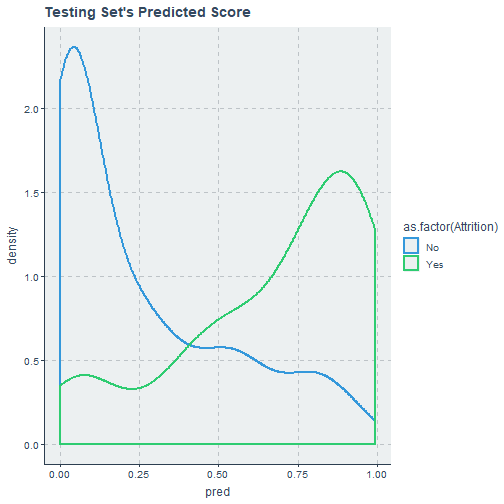
\includegraphics{IBM-HR-Analytics-ML-Classification_files/figure-latex/unnamed-chunk-27-1.pdf}

We want a threshold number which have the highest accuracy and the
smallest false negative rate. By looking at the graph, the threshold
should be around 0.3 or 0.4. Now we will try both values to see the
results

\begin{Shaded}
\begin{Highlighting}[]
\NormalTok{pred_round <-}\StringTok{ }\KeywordTok{as.factor}\NormalTok{(}\KeywordTok{ifelse}\NormalTok{(pred }\OperatorTok{>=}\StringTok{ }\FloatTok{0.3}\NormalTok{, }\StringTok{"Yes"}\NormalTok{, }\StringTok{"No"}\NormalTok{))}
\KeywordTok{confusionMatrix}\NormalTok{(pred_round, data_test}\OperatorTok{$}\NormalTok{Attrition, }\DataTypeTok{positive =} \StringTok{"Yes"}\NormalTok{)}
\end{Highlighting}
\end{Shaded}

\begin{verbatim}
## Confusion Matrix and Statistics
## 
##           Reference
## Prediction  No Yes
##        No  159   7
##        Yes  78  50
##                                          
##                Accuracy : 0.7109         
##                  95% CI : (0.6554, 0.762)
##     No Information Rate : 0.8061         
##     P-Value [Acc > NIR] : 1              
##                                          
##                   Kappa : 0.3721         
##                                          
##  Mcnemar's Test P-Value : 3.136e-14      
##                                          
##             Sensitivity : 0.8772         
##             Specificity : 0.6709         
##          Pos Pred Value : 0.3906         
##          Neg Pred Value : 0.9578         
##              Prevalence : 0.1939         
##          Detection Rate : 0.1701         
##    Detection Prevalence : 0.4354         
##       Balanced Accuracy : 0.7740         
##                                          
##        'Positive' Class : Yes            
## 
\end{verbatim}

\begin{Shaded}
\begin{Highlighting}[]
\NormalTok{pred_round <-}\StringTok{ }\KeywordTok{as.factor}\NormalTok{(}\KeywordTok{ifelse}\NormalTok{(pred }\OperatorTok{>=}\StringTok{ }\FloatTok{0.4}\NormalTok{, }\StringTok{"Yes"}\NormalTok{, }\StringTok{"No"}\NormalTok{))}
\KeywordTok{confusionMatrix}\NormalTok{(pred_round, data_test}\OperatorTok{$}\NormalTok{Attrition, }\DataTypeTok{positive =} \StringTok{"Yes"}\NormalTok{)}
\end{Highlighting}
\end{Shaded}

\begin{verbatim}
## Confusion Matrix and Statistics
## 
##           Reference
## Prediction  No Yes
##        No  173  10
##        Yes  64  47
##                                           
##                Accuracy : 0.7483          
##                  95% CI : (0.6946, 0.7969)
##     No Information Rate : 0.8061          
##     P-Value [Acc > NIR] : 0.9939          
##                                           
##                   Kappa : 0.4078          
##                                           
##  Mcnemar's Test P-Value : 7.223e-10       
##                                           
##             Sensitivity : 0.8246          
##             Specificity : 0.7300          
##          Pos Pred Value : 0.4234          
##          Neg Pred Value : 0.9454          
##              Prevalence : 0.1939          
##          Detection Rate : 0.1599          
##    Detection Prevalence : 0.3776          
##       Balanced Accuracy : 0.7773          
##                                           
##        'Positive' Class : Yes             
## 
\end{verbatim}

The threshold value of 0.3 and 0.4 successfully decreasing the False
Negative count of the prediction, thus increasing the Sensitivity of the
data. It is also increasing the number of True Positive count of the
prediction. Good sign!

The drawback of adjusting the threshold in our prediction is our model
failed to predict the True Negative count. But if we think the False
Positive is not a big deal, then it should not be a problem.

\hypertarget{knn-with-caret}{%
\subsection{KNN with caret()}\label{knn-with-caret}}

KNN or k-nearest neighbors is a non-parametric method that can be used
for classification. We will try to predict using this method and compare
the performance with the Logistic Regression.

KNN is only work for predictor with numerical values, so we will select
the numerical columns only.

First, we will divide our dataset into 80\% in train data and 20\% in
test data. We will using set.seed() function to make sure that R produce
the same random number to make this report is reproducible.

\begin{Shaded}
\begin{Highlighting}[]
\KeywordTok{RNGkind}\NormalTok{(}\DataTypeTok{sample.kind =} \StringTok{"Rounding"}\NormalTok{)}
\end{Highlighting}
\end{Shaded}

\begin{verbatim}
## Warning in RNGkind(sample.kind = "Rounding"): non-uniform 'Rounding' sampler
## used
\end{verbatim}

\begin{Shaded}
\begin{Highlighting}[]
\KeywordTok{set.seed}\NormalTok{(}\DecValTok{18}\NormalTok{)}
\NormalTok{ind <-}\StringTok{ }\NormalTok{dataHR_num}\OperatorTok{$}\NormalTok{Attrition }\OperatorTok\StringTok{ }
\StringTok{  }\KeywordTok{createDataPartition}\NormalTok{(}\DataTypeTok{p =} \FloatTok{0.8}\NormalTok{, }\DataTypeTok{list =} \OtherTok{FALSE}\NormalTok{)}
\NormalTok{train_caret  <-}\StringTok{ }\NormalTok{dataHR_num[ind, ]}
\NormalTok{test_caret <-}\StringTok{ }\NormalTok{dataHR_num[}\OperatorTok{-}\NormalTok{ind, ]}
\end{Highlighting}
\end{Shaded}

I will be using caret package to predict with KNN. After data splited
into training set and train set, I am using k-Fold Cross-Validation
parameter in the train() function. The data pre-processing of Centering
and Scaling will be done in the trainControl() function.

The k-Fold Cross-Validation parameter will be set all to 10. Data
imbalanced will be handled using sampling method in trainControl()
function, I will try all the options available to compare how the
different sampling method will perform.

The k values of KNN method will be set with the tuneGrid in train()
function. The function will take the best k value automatically to be
used in test set which has the best ROC, from metric options.

\begin{Shaded}
\begin{Highlighting}[]
\KeywordTok{sqrt}\NormalTok{(}\KeywordTok{nrow}\NormalTok{(dataHR))}
\end{Highlighting}
\end{Shaded}

\begin{verbatim}
## [1] 38.34058
\end{verbatim}

The rule of thumb of k value in KNN is the square root of number of rows
in dataset. I will iterate from 1 to 50 for the k values of KNN in the
tuneGrid. The function will take the best k value that produce the
highest value of Sensitivity. The Sensitivity parameter is chosen
according to our company objective.

The imbalanced data will be handled using several sampling method:
Upsampling, Downsampling, SMOTE, ROSE.

\begin{Shaded}
\begin{Highlighting}[]
\NormalTok{model_imbalanced <-}\StringTok{ }\KeywordTok{train}\NormalTok{(}
\NormalTok{  Attrition }\OperatorTok{~}\NormalTok{., }\DataTypeTok{data =}\NormalTok{ train_caret, }\DataTypeTok{method =} \StringTok{"knn"}\NormalTok{,}
  \DataTypeTok{trControl =} \KeywordTok{trainControl}\NormalTok{(}\DataTypeTok{method =} \StringTok{"cv"}\NormalTok{,}
                           \DataTypeTok{number =} \DecValTok{10}\NormalTok{,}
                           \DataTypeTok{classProbs =} \OtherTok{TRUE}\NormalTok{,}
                           \DataTypeTok{summaryFunction=}\NormalTok{twoClassSummary),}
  \DataTypeTok{preProcess =} \KeywordTok{c}\NormalTok{(}\StringTok{"center"}\NormalTok{,}\StringTok{"scale"}\NormalTok{),}
  \DataTypeTok{metric =} \StringTok{"Sens"}\NormalTok{,}
  \DataTypeTok{tuneGrid =} \KeywordTok{expand.grid}\NormalTok{(}\DataTypeTok{k =} \DecValTok{1}\OperatorTok{:}\DecValTok{50}\NormalTok{)}
\NormalTok{  )}

\NormalTok{model_upsampling <-}\StringTok{ }\KeywordTok{train}\NormalTok{(}
\NormalTok{  Attrition }\OperatorTok{~}\NormalTok{., }\DataTypeTok{data =}\NormalTok{ train_caret, }\DataTypeTok{method =} \StringTok{"knn"}\NormalTok{,}
  \DataTypeTok{trControl =} \KeywordTok{trainControl}\NormalTok{(}\DataTypeTok{method =} \StringTok{"cv"}\NormalTok{,}
                           \DataTypeTok{number =} \DecValTok{10}\NormalTok{,}
                           \DataTypeTok{sampling =} \StringTok{"up"}\NormalTok{,}
                           \DataTypeTok{classProbs =} \OtherTok{TRUE}\NormalTok{,}
                           \DataTypeTok{summaryFunction=}\NormalTok{twoClassSummary),}
  \DataTypeTok{preProcess =} \KeywordTok{c}\NormalTok{(}\StringTok{"center"}\NormalTok{,}\StringTok{"scale"}\NormalTok{),}
  \DataTypeTok{metric =} \StringTok{"Sens"}\NormalTok{,}
  \DataTypeTok{tuneGrid =} \KeywordTok{expand.grid}\NormalTok{(}\DataTypeTok{k =} \DecValTok{1}\OperatorTok{:}\DecValTok{50}\NormalTok{)}
\NormalTok{  )}

\NormalTok{model_downsampling <-}\StringTok{ }\KeywordTok{train}\NormalTok{(}
\NormalTok{  Attrition }\OperatorTok{~}\NormalTok{., }\DataTypeTok{data =}\NormalTok{ train_caret, }\DataTypeTok{method =} \StringTok{"knn"}\NormalTok{,}
  \DataTypeTok{trControl =} \KeywordTok{trainControl}\NormalTok{(}\DataTypeTok{method =} \StringTok{"cv"}\NormalTok{,}
                           \DataTypeTok{number =} \DecValTok{10}\NormalTok{,}
                           \DataTypeTok{sampling =} \StringTok{"down"}\NormalTok{,}
                           \DataTypeTok{classProbs =} \OtherTok{TRUE}\NormalTok{,}
                           \DataTypeTok{summaryFunction=}\NormalTok{twoClassSummary),}
  \DataTypeTok{preProcess =} \KeywordTok{c}\NormalTok{(}\StringTok{"center"}\NormalTok{,}\StringTok{"scale"}\NormalTok{),}
  \DataTypeTok{metric =} \StringTok{"Sens"}\NormalTok{,}
  \DataTypeTok{tuneGrid =} \KeywordTok{expand.grid}\NormalTok{(}\DataTypeTok{k =} \DecValTok{1}\OperatorTok{:}\DecValTok{50}\NormalTok{)}
\NormalTok{  )}

\NormalTok{model_smote<-}\StringTok{ }\KeywordTok{train}\NormalTok{(}
\NormalTok{  Attrition }\OperatorTok{~}\NormalTok{., }\DataTypeTok{data =}\NormalTok{ train_caret, }\DataTypeTok{method =} \StringTok{"knn"}\NormalTok{,}
  \DataTypeTok{trControl =} \KeywordTok{trainControl}\NormalTok{(}\DataTypeTok{method =} \StringTok{"cv"}\NormalTok{,}
                           \DataTypeTok{number =} \DecValTok{10}\NormalTok{,}
                           \DataTypeTok{sampling =} \StringTok{"smote"}\NormalTok{,}
                           \DataTypeTok{classProbs =} \OtherTok{TRUE}\NormalTok{,}
                           \DataTypeTok{summaryFunction=}\NormalTok{twoClassSummary),}
  \DataTypeTok{preProcess =} \KeywordTok{c}\NormalTok{(}\StringTok{"center"}\NormalTok{,}\StringTok{"scale"}\NormalTok{),}
  \DataTypeTok{metric =} \StringTok{"Sens"}\NormalTok{,}
  \DataTypeTok{tuneGrid =} \KeywordTok{expand.grid}\NormalTok{(}\DataTypeTok{k =} \DecValTok{1}\OperatorTok{:}\DecValTok{50}\NormalTok{)}
\NormalTok{  )}
\end{Highlighting}
\end{Shaded}

\begin{verbatim}
## Warning: package 'DMwR' was built under R version 3.6.2
\end{verbatim}

\begin{verbatim}
## Loading required package: grid
\end{verbatim}

\begin{verbatim}
## Registered S3 method overwritten by 'xts':
##   method     from
##   as.zoo.xts zoo
\end{verbatim}

\begin{verbatim}
## Registered S3 method overwritten by 'quantmod':
##   method            from
##   as.zoo.data.frame zoo
\end{verbatim}

\begin{Shaded}
\begin{Highlighting}[]
\NormalTok{model_rose<-}\StringTok{ }\KeywordTok{train}\NormalTok{(}
\NormalTok{  Attrition }\OperatorTok{~}\NormalTok{., }\DataTypeTok{data =}\NormalTok{ train_caret, }\DataTypeTok{method =} \StringTok{"knn"}\NormalTok{,}
  \DataTypeTok{trControl =} \KeywordTok{trainControl}\NormalTok{(}\DataTypeTok{method =} \StringTok{"cv"}\NormalTok{,}
                           \DataTypeTok{number =} \DecValTok{10}\NormalTok{,}
                           \DataTypeTok{sampling =} \StringTok{"rose"}\NormalTok{,}
                           \DataTypeTok{classProbs =} \OtherTok{TRUE}\NormalTok{,}
                           \DataTypeTok{summaryFunction=}\NormalTok{twoClassSummary),}
  \DataTypeTok{preProcess =} \KeywordTok{c}\NormalTok{(}\StringTok{"center"}\NormalTok{,}\StringTok{"scale"}\NormalTok{),}
  \DataTypeTok{metric =} \StringTok{"Sens"}\NormalTok{,}
  \DataTypeTok{tuneGrid =} \KeywordTok{expand.grid}\NormalTok{(}\DataTypeTok{k =} \DecValTok{1}\OperatorTok{:}\DecValTok{50}\NormalTok{)}
\NormalTok{  )}
\end{Highlighting}
\end{Shaded}

No we will make a prediction with our created models into the test
dataset and we will save the results into appropiate objects.

\begin{Shaded}
\begin{Highlighting}[]
\NormalTok{pred_imbalanced <-}\StringTok{ }\NormalTok{model_imbalanced }\OperatorTok\StringTok{ }
\StringTok{  }\KeywordTok{predict}\NormalTok{(test_caret)}
\NormalTok{pred_upsampling <-}\StringTok{ }\NormalTok{model_upsampling }\OperatorTok\StringTok{ }
\StringTok{  }\KeywordTok{predict}\NormalTok{(test_caret)}
\NormalTok{pred_downsampling <-}\StringTok{ }\NormalTok{model_downsampling }\OperatorTok\StringTok{ }
\StringTok{  }\KeywordTok{predict}\NormalTok{(test_caret)}
\NormalTok{pred_smote <-}\StringTok{ }\NormalTok{model_smote }\OperatorTok\StringTok{ }
\StringTok{  }\KeywordTok{predict}\NormalTok{(test_caret)}
\NormalTok{pred_rose <-}\StringTok{ }\NormalTok{model_rose }\OperatorTok\StringTok{ }
\StringTok{  }\KeywordTok{predict}\NormalTok{(test_caret)}
\end{Highlighting}
\end{Shaded}

\begin{Shaded}
\begin{Highlighting}[]
\KeywordTok{confusionMatrix}\NormalTok{(pred_imbalanced, test_caret}\OperatorTok{$}\NormalTok{Attrition)}
\end{Highlighting}
\end{Shaded}

\begin{verbatim}
## Confusion Matrix and Statistics
## 
##           Reference
## Prediction Yes  No
##        Yes  15  38
##        No   32 208
##                                           
##                Accuracy : 0.7611          
##                  95% CI : (0.7081, 0.8088)
##     No Information Rate : 0.8396          
##     P-Value [Acc > NIR] : 0.9998          
##                                           
##                   Kappa : 0.1566          
##                                           
##  Mcnemar's Test P-Value : 0.5501          
##                                           
##             Sensitivity : 0.31915         
##             Specificity : 0.84553         
##          Pos Pred Value : 0.28302         
##          Neg Pred Value : 0.86667         
##              Prevalence : 0.16041         
##          Detection Rate : 0.05119         
##    Detection Prevalence : 0.18089         
##       Balanced Accuracy : 0.58234         
##                                           
##        'Positive' Class : Yes             
## 
\end{verbatim}

\begin{Shaded}
\begin{Highlighting}[]
\KeywordTok{confusionMatrix}\NormalTok{(pred_upsampling, test_caret}\OperatorTok{$}\NormalTok{Attrition, }\DataTypeTok{positive =} \StringTok{"Yes"}\NormalTok{)}
\end{Highlighting}
\end{Shaded}

\begin{verbatim}
## Confusion Matrix and Statistics
## 
##           Reference
## Prediction Yes  No
##        Yes  29 102
##        No   18 144
##                                           
##                Accuracy : 0.5904          
##                  95% CI : (0.5318, 0.6473)
##     No Information Rate : 0.8396          
##     P-Value [Acc > NIR] : 1               
##                                           
##                   Kappa : 0.1175          
##                                           
##  Mcnemar's Test P-Value : 3.541e-14       
##                                           
##             Sensitivity : 0.61702         
##             Specificity : 0.58537         
##          Pos Pred Value : 0.22137         
##          Neg Pred Value : 0.88889         
##              Prevalence : 0.16041         
##          Detection Rate : 0.09898         
##    Detection Prevalence : 0.44710         
##       Balanced Accuracy : 0.60119         
##                                           
##        'Positive' Class : Yes             
## 
\end{verbatim}

\begin{Shaded}
\begin{Highlighting}[]
\KeywordTok{confusionMatrix}\NormalTok{(pred_downsampling, test_caret}\OperatorTok{$}\NormalTok{Attrition, }\DataTypeTok{positive =} \StringTok{"Yes"}\NormalTok{)}
\end{Highlighting}
\end{Shaded}

\begin{verbatim}
## Confusion Matrix and Statistics
## 
##           Reference
## Prediction Yes  No
##        Yes  26 101
##        No   21 145
##                                           
##                Accuracy : 0.5836          
##                  95% CI : (0.5249, 0.6407)
##     No Information Rate : 0.8396          
##     P-Value [Acc > NIR] : 1               
##                                           
##                   Kappa : 0.0845          
##                                           
##  Mcnemar's Test P-Value : 8.532e-13       
##                                           
##             Sensitivity : 0.55319         
##             Specificity : 0.58943         
##          Pos Pred Value : 0.20472         
##          Neg Pred Value : 0.87349         
##              Prevalence : 0.16041         
##          Detection Rate : 0.08874         
##    Detection Prevalence : 0.43345         
##       Balanced Accuracy : 0.57131         
##                                           
##        'Positive' Class : Yes             
## 
\end{verbatim}

\begin{Shaded}
\begin{Highlighting}[]
\KeywordTok{confusionMatrix}\NormalTok{(pred_smote, test_caret}\OperatorTok{$}\NormalTok{Attrition, }\DataTypeTok{positive =} \StringTok{"Yes"}\NormalTok{)}
\end{Highlighting}
\end{Shaded}

\begin{verbatim}
## Confusion Matrix and Statistics
## 
##           Reference
## Prediction Yes  No
##        Yes  23  82
##        No   24 164
##                                           
##                Accuracy : 0.6382          
##                  95% CI : (0.5803, 0.6933)
##     No Information Rate : 0.8396          
##     P-Value [Acc > NIR] : 1               
##                                           
##                   Kappa : 0.1041          
##                                           
##  Mcnemar's Test P-Value : 3.089e-08       
##                                           
##             Sensitivity : 0.4894          
##             Specificity : 0.6667          
##          Pos Pred Value : 0.2190          
##          Neg Pred Value : 0.8723          
##              Prevalence : 0.1604          
##          Detection Rate : 0.0785          
##    Detection Prevalence : 0.3584          
##       Balanced Accuracy : 0.5780          
##                                           
##        'Positive' Class : Yes             
## 
\end{verbatim}

\begin{Shaded}
\begin{Highlighting}[]
\KeywordTok{confusionMatrix}\NormalTok{(pred_rose, test_caret}\OperatorTok{$}\NormalTok{Attrition, }\DataTypeTok{positive =} \StringTok{"Yes"}\NormalTok{)}
\end{Highlighting}
\end{Shaded}

\begin{verbatim}
## Confusion Matrix and Statistics
## 
##           Reference
## Prediction Yes  No
##        Yes  27  81
##        No   20 165
##                                           
##                Accuracy : 0.6553          
##                  95% CI : (0.5978, 0.7096)
##     No Information Rate : 0.8396          
##     P-Value [Acc > NIR] : 1               
##                                           
##                   Kappa : 0.1608          
##                                           
##  Mcnemar's Test P-Value : 2.369e-09       
##                                           
##             Sensitivity : 0.57447         
##             Specificity : 0.67073         
##          Pos Pred Value : 0.25000         
##          Neg Pred Value : 0.89189         
##              Prevalence : 0.16041         
##          Detection Rate : 0.09215         
##    Detection Prevalence : 0.36860         
##       Balanced Accuracy : 0.62260         
##                                           
##        'Positive' Class : Yes             
## 
\end{verbatim}

We will calculate the performance differences statistically.

\begin{Shaded}
\begin{Highlighting}[]
\NormalTok{resamps <-}\StringTok{ }\KeywordTok{resamples}\NormalTok{(}\KeywordTok{list}\NormalTok{(}\DataTypeTok{Imbalanced =}\NormalTok{ model_imbalanced,}
                          \DataTypeTok{Upsampling =}\NormalTok{ model_upsampling,}
                          \DataTypeTok{Downsampling =}\NormalTok{ model_downsampling,}
                          \DataTypeTok{SMOTE =}\NormalTok{ model_smote,}
                          \DataTypeTok{ROSE =}\NormalTok{ model_rose))}
\end{Highlighting}
\end{Shaded}

\begin{Shaded}
\begin{Highlighting}[]
\NormalTok{resamps}\OperatorTok{$}\NormalTok{values }\OperatorTok
\StringTok{  }\KeywordTok{select}\NormalTok{(Resample, }
         \DataTypeTok{Imbalanced =} \StringTok{`}\DataTypeTok{Imbalanced~Sens}\StringTok{`}\NormalTok{, }
         \DataTypeTok{Upsampling =} \StringTok{`}\DataTypeTok{Upsampling~Sens}\StringTok{`}\NormalTok{, }
         \DataTypeTok{Downsampling =} \StringTok{`}\DataTypeTok{Downsampling~Sens}\StringTok{`}\NormalTok{, }
         \DataTypeTok{SMOTE =} \StringTok{`}\DataTypeTok{SMOTE~Sens}\StringTok{`}\NormalTok{, }
         \DataTypeTok{ROSE =} \StringTok{`}\DataTypeTok{ROSE~Sens}\StringTok{`}\NormalTok{)}
\end{Highlighting}
\end{Shaded}

\begin{verbatim}
##    Resample Imbalanced Upsampling Downsampling     SMOTE      ROSE
## 1    Fold01  0.2105263  0.5789474    0.6315789 0.5789474 0.6315789
## 2    Fold02  0.1578947  0.6315789    0.6315789 0.5263158 0.5789474
## 3    Fold03  0.2105263  0.7894737    0.7368421 0.6315789 0.6842105
## 4    Fold04  0.2631579  0.4210526    0.4736842 0.6315789 0.7368421
## 5    Fold05  0.1052632  0.7894737    0.8421053 0.4210526 0.5263158
## 6    Fold06  0.4210526  0.6842105    0.3684211 0.4736842 0.5789474
## 7    Fold07  0.2631579  0.6842105    0.6842105 0.6315789 0.7368421
## 8    Fold08  0.5263158  0.5789474    0.6842105 0.3684211 0.6315789
## 9    Fold09  0.2105263  0.4736842    0.7368421 0.6842105 0.5789474
## 10   Fold10  0.3684211  0.9473684    0.6315789 0.6842105 0.7894737
\end{verbatim}

\begin{Shaded}
\begin{Highlighting}[]
\KeywordTok{bwplot}\NormalTok{(resamps, }\DataTypeTok{layout =} \KeywordTok{c}\NormalTok{(}\DecValTok{3}\NormalTok{, }\DecValTok{1}\NormalTok{))}
\end{Highlighting}
\end{Shaded}

\includegraphics{IBM-HR-Analytics-ML-Classification_files/figure-latex/unnamed-chunk-42-1.pdf}

From the table and the chart above, we can conclude that, in general,
Upsampling producted the highest Sensitivity value of our model. It
doesn't mean that Upsampling is always the best for all model and all
situation. But in our case, because we focus on the Sensitivity value,
the Upsampling method gives us the best result.

\hypertarget{conclusion}{%
\section{Conclusion}\label{conclusion}}

Our model summary: 1. Logistic Regression with default threshold
(\textgreater{} 0.5) Accuracy: 0.7721 Sensitivity : 0.7368 2. Logistic
Regression with threshold \textgreater{} 0.3 Accuracy: 0.7075
Sensitivity: 0.8772 3. Logistic Regression with threshold \textgreater{}
0.4 Accuracy: 0.7381 Sensitivity: 0.8070 4. KNN with Imbalanced Data
Accuracy: 0.7611 Sensitivity: 0.31915 5. KNN with Unsampling Accuracy:
0.5904 Sensitivity: 0.61702 6. KNN with Downsampling Accuracy: 0.5836
Sensitivity: 0.55319 7. KNN with SMOTE Accuracy: 0.6382 Sensitivity:
0.4894 8. KNN with ROSE Accuracy: 0.6553 Sensitivity: 0.5745

Our prediction with the KNN method, all produces both Accuracy and
Sensitivity score lower than the Logistic Regression Model. Maybe it is
because we only use the numerical value type of predictors in the KNN.
We may lose some valuable information that may contain in the
categorical predictors.

With both numerical and categorical type of columns included in the
Logistic Regression model, it produces a better value than the KNN. If
our objective is decreasing the False Negative as defined by the
business objective, we will choose \emph{Logistic Regression with
threshold \textgreater{} 0.3} for our model.

\end{document}
